\documentclass{article}
\usepackage[utf8]{inputenc}
\RequirePackage{amsmath,amssymb}
\RequirePackage{xcolor,graphicx}
\RequirePackage{tikz,pgfplots}
\usetikzlibrary{shapes,arrows,positioning,matrix,backgrounds,fit}
\usepackage{hyperref}
\tikzstyle{rec} = [ rectangle, minimum width=3cm, minimum height=1cm, text centered,text width=2.3cm, draw=black]

% \title{inlab-11}
% \author{yashkhem1 }
% \date{October 2018}

\begin{document}

\begin{center}
    \LARGE{YAY - Inlab 11}\\
    \vspace{20pt}
    \large{170050025(33.33\%),170050055(33.33\%),170070015(33.33\%)}\\
    \vspace{10pt}
    \large{October 22, 2018}\\
    \vspace{30pt}
    \textbf{Declaration}\\
    \end{center}
    
    I acknowledge and understand that plagiarism is wrong. This project is my ownwork, or my group’s own unique group project. I acknowledge that copying some-one else’s work, or part of it, is wrong, and that submitting identical work to others constitutes a form of plagiarism.
    \section{Work Done So Far}
    We have successfully built the Linux Client which can upload the files that are present in the current working directory but not present in the server and can download files present in the server but not present in the working directory.
    {\color{blue}{\cite{Site1}}}We have achieved this by implementing REST framework in Django. {\color{blue}{\cite{Site2}}} 
    
    
    \section{System Architecture Using TikZ}
    \begin{center}
        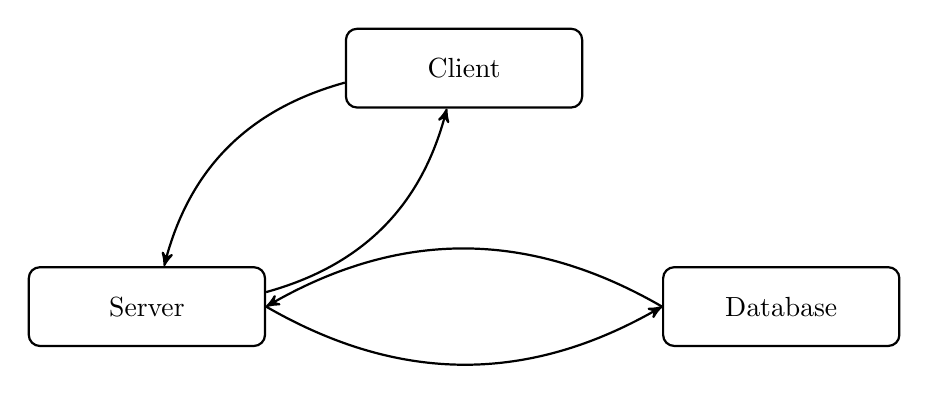
\begin{tikzpicture}[->,>=stealth',auto,node distance=3cm,
  thick,main node/.style={circle,draw,font=\sffamily\Large\bfseries}]
          \node (Client) [rounded corners, rec] {Client};
          \node (Server) [rounded corners,rec, below left = 2cm and 1 cm of Client, draw=black] {Server};
          \node (Database) [rounded corners, rec, below right = 2cm and 1 cm of Client, draw=black] {Database};
          
           \path[every node/.style={font=\sffamily\small}]
            (Client) edge[bend right] node [left] {} (Server)
            (Server) edge[bend right] node [right] {} (Client)
            (Database.west) edge[bend right] node[left] {} (Server.east)
            (Server.east) edge[bend right] node[right] {} (Database.west);
         \end{tikzpicture}
    \end{center}
    \section{Result and Analysis}
    \begin{figure}[H]
        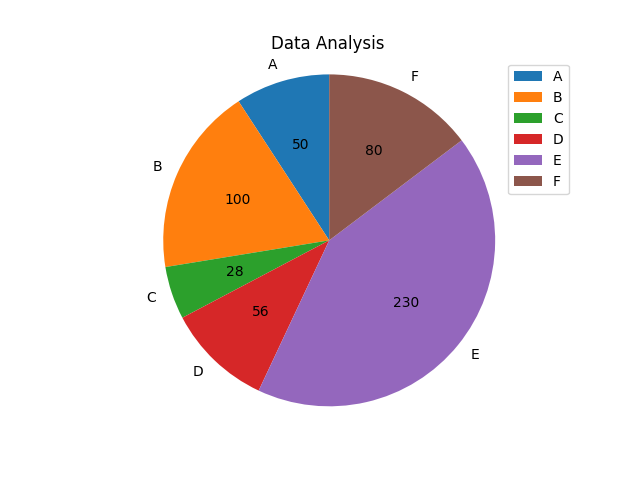
\includegraphics[width=\linewidth]{Data.png}
        \caption{Data Analysis}
        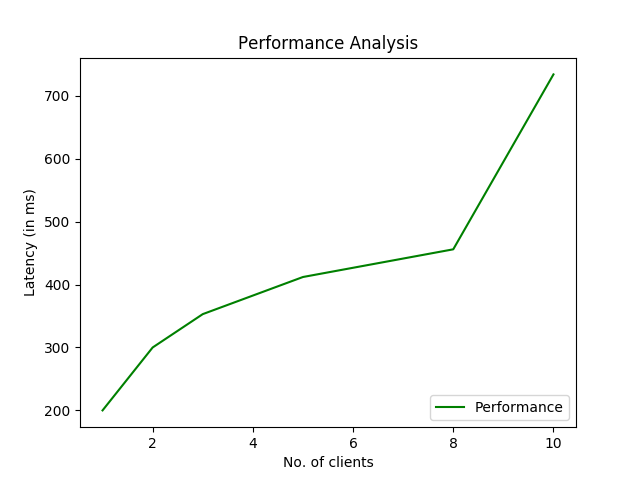
\includegraphics[width=\linewidth]{Performance.png}
        \caption{Performance Data Analysis}
    \end{figure}
    \newpage
    \section{Future Work}
    We plan to create a Web Client which displays the files present in the server for the user. We also plan to create an android app for the same.
    
    

    \begin{thebibliography}{9}
    \bibitem{Site1} 
    Inspired from Google. Available \href{www.google.com}{\color{blue}{here}}
     
    \bibitem{Site2} 
    Youtube Videos at \href{https://www.youtube.com/watch?v=dQw4w9WgXcQ}{\color{blue}{this link}}

    \end{thebibliography}


    
    
    
    %%https://www.django-rest-framework.org/api-guide/parsers/

\end{document}
